\section{Co-Packaged Protocol and Baseline Encapsulations}\label{sec:design}

\begin{figure}[t]
  \centering
  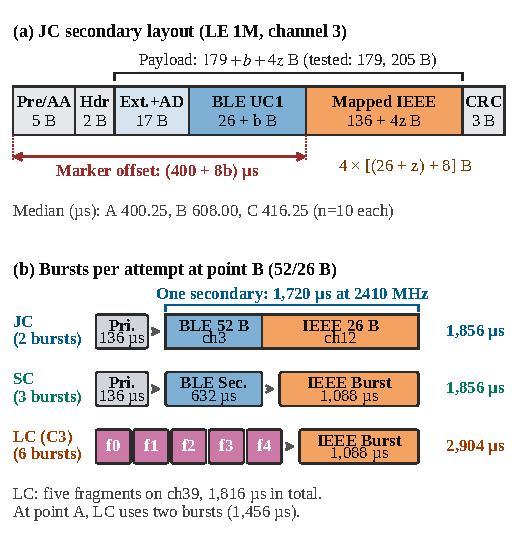
\includegraphics[width=\columnwidth]{figures/fig-uc1-layout-bursts.pdf}
  \caption{Unified compact (\proto{}) co-packaged secondary PDU layout and single-attempt burst comparison across \modejc{}, \modesc{}, and \modelc{}: (a) \texttt{AUX\_ADV\_IND} byte budget, BlueBee $4\times$ mapping expansion, and deterministic $\num{400}+8b\,\si{\micro\second}$ marker offset; (b) per-attempt burst structures at Point~B ($52/26$\,B, where \modejc{} uses one \SI{1720}{\micro\second} secondary burst and \modelc{} requires five \fragproto{} fragments on ch39).}
  \label{fig:layout}
\end{figure}

\subsection{Encapsulation Modes and Byte/Waveform Budgets}\label{sec:design_modes}

The transmitter schedules attempts in \SI{500}{ms} slots ($T_{\text{slot}}{=}\SI{500}{ms}$) toward a \ble{} chain and an \stdfour{} chain; in P4, successive logical tasks start six slots apart (\SI{3}{s}). Each logical task $(\texttt{run\_id}, \texttt{command\_id})$ is sent open-loop without ACKs across $K$ planned attempts under a fixed-$K$ rule or a per-task waveform budget cap $Q$ (\si{\micro\second}), consuming a strictly increasing \texttt{slot\_index}. Fig.~\ref{fig:layout} contrasts three modes under identical task semantics: \modejc{} sends $2$ bursts/attempt---one primary \texttt{ADV\_EXT\_IND} (\SI{136}{\micro\second}) and one co-packaged \texttt{AUX\_ADV\_IND} on \ble{} ch3 / \stdfour{} ch12 (\SI{2410}{MHz}); \modesc{} sends $3$ bursts/attempt---primary, \ble{}-only secondary on ch3, and standalone BlueBee-mapped \stdfour{} burst on ch12; and \modelc{} sends $F{+}1$ bursts/attempt---$F$ legacy \ble{} frames on ch39 (\SI{2480}{MHz}) plus $1$ standalone \stdfour{} burst on ch12.

Each side independently frames and verifies a $(26{+}n)$-byte little-endian \proto{} record ($n{=}b$ on \ble{}, $n{=}z$ on \stdfour{}), comprising a \SI{24}{B} fixed header (\texttt{magic=0xC1}, explicit \texttt{version\_type} \texttt{0x10} time-update or \texttt{0x11} command, \texttt{run\_id}, \texttt{slot\_index}, \texttt{period\_ms}, \texttt{command\_id}, \texttt{target\_id}, \texttt{opcode}, \texttt{arg}, relative validity/execution offsets, and \texttt{extra\_len}), $n$\,B of side-specific \texttt{extra\_payload}, and a \SI{2}{B} \texttt{CRC-16/CCITT-FALSE}. In \modejc{}, extended-advertising and AD headers occupy \SI{17}{B} and the BlueBee region occupies $4(26{+}z{+}8){=}136{+}4z$\,B (including \SI{8}{B} \stdfour{} framing), yielding secondary PDU payload length
\begin{equation}\label{eq:sec_payload}
  L_{\text{sec}}(b,z) = 17 + (26 + b) + (136 + 4z) = 179 + b + 4z~\text{B}.
\end{equation}
The \SI{255}{B} PDU ceiling gives an arithmetic limit $b{+}4z\le 76$, whereas our frozen Phase-1 working domain enforces $0\le b\le 26$, $0\le z\le 6$, and $b{+}4z\le 26$ ($b{=}26$ and $z{=}6$ cannot be combined). We test three complete (\ble{}/\stdfour{}) record pairs---Point~A ($26/26$\,B, \SI{179}{B} payload), Point~B ($52/26$\,B, \SI{205}{B}), and Point~C ($28/32$\,B, \SI{205}{B})---plus Point~B1 ($27/26$\,B) for the \SI{27}{B} direct legacy ceiling.

At LE~1M, single-attempt submitted waveform proxies (\si{\micro\second}, excluding silence and tuning guards; Table~\ref{tab:budget}) follow
\begin{align}
  C_{\modejc}(b,z) &= C_{\modesc}(b,z) = 1648 + 8b + 32z,\label{eq:cost_jc_sc}\\
  C_{\modelc}(b,z) &=
  \begin{cases}
    8(182 + b + 4z), & b \le 1,\\
    8(35F + 162 + b + 4z), & b \ge 2.
  \end{cases}\label{eq:cost_lc}
\end{align}
For $b\le 1$, \modelc{} carries the \ble{} record in one Manufacturer AD frame ($F{=}1$); for $b\ge 2$, each fragment incurs \SI{20}{B} of legacy framing overhead and carries a \SI{15}{B} \fragproto{} header followed by up to \SI{12}{B} of record data, requiring $F{=}\lceil(26{+}b)/12\rceil$ fragments ($F{=}5$ at Point~B). Thus $C_{\modejc}{=}C_{\modesc}$ for all $(b,z)$ while \modejc{} cuts bursts from $3$ to $2$. Under cap $Q$, each mode gets $K_m{=}\lfloor Q/C_m\rfloor$ attempts, with unused budget $Q{-}K_m C_m$ reported explicitly.

% ============================================================
%  Table I: UC1 / C3 Byte Layout & Per-Attempt Waveform Proxy Budget
%  ITCA / IEEEtran rule: letter table footnotes (a, b, ...); period after caption.
% ============================================================
\begin{table}[t]
\centering
\caption{Byte Layout, Per-Attempt Submitted Waveform Proxy Budget, and Wired Feeder Verification Across Representative Workloads.}
\label{tab:budget}
\setlength{\tabcolsep}{2.2pt}
\scriptsize
\begin{tabular}{@{}lccccccc@{}}
\toprule
\textbf{Point} & \textbf{Rec.} & \textbf{Map} & \textbf{\modejc{} Sec.} & \multicolumn{3}{c}{\textbf{Bursts / Proxy (\si{\micro\second})}} & \textbf{H1 Med.} \\
\cmidrule(lr){5-7}
$(b,z)$ & B/Z & (B) & (B) & \modejc{} & \modesc{} & \modelc{} ($F$) & (\si{\micro\second}) \\
\midrule
A $(0,0)$   & 26/26 & 136 & 179 & 2/\num{1648} & 3/\num{1648} & 2/\num{1456} (1) & 400.25 \\
B1 $(1,0)$  & 27/26 & 136 & 180$^{\mathrm{a}}$ & 2/\num{1656}$^{\mathrm{a}}$ & 3/\num{1656}$^{\mathrm{a}}$ & 2/\num{1464} (1) & --- \\
C $(2,6)$   & 28/32 & 160 & 205 & 2/\num{1856} & 3/\num{1856} & 4/\num{2344} (3) & 416.25 \\
B $(26,0)$  & 52/26 & 136 & 205 & 2/\num{1856} & 3/\num{1856} & 6/\num{2904} (5) & 608.00 \\
\bottomrule
\end{tabular}
\par\smallskip
\raggedright\scriptsize
All 10 tested \texttt{R0} branches (runs 2702--2710, 2718) achieved $10/10$ joint resolution. $F$: legacy \ble{} frames/attempt ($F{=}1$ for $b\le 1$; $F{=}\lceil(26{+}b)/12\rceil$ \fragproto{} fragments for $b\ge 2$, plus $1$ \stdfour{} burst). $^{\mathrm{a}}$Formula values; at B1 only the \SI{27}{B} direct \modelc{} ceiling (run 2710) was captured. Shared-IQ H1 medians ($n{=}10$ each) validate $400{+}8b\,\si{\micro\second}$, not cross-device clock error.
\end{table}


\subsection{Deterministic Offset, Retry Semantics, and \fragproto{} Reassembly}\label{sec:design_semantics}

\proto{} anchors $\texttt{ref\_tick\_ms}=\texttt{slot\_index}\times\texttt{period\_ms}$ to the secondary \ble{} preamble in \modejc{}. Because the BlueBee region begins at payload byte $43{+}b$ after the \SI{5}{B} preamble/access address and \SI{2}{B} PDU header, the structural marker offset is
\begin{equation}\label{eq:offset}
  \Delta t_{\text{marker}}(b) = (5 + 2 + 43 + b)\times \SI{8}{\micro\second} = 400 + 8b~\si{\micro\second}.
\end{equation}
Keeping fixed record overhead at \SI{26}{B} requires the \stdfour{} receiver to read $b$ from the pre-shared run configuration; missing or mismatched layout metadata forces $\texttt{timing\_eligible}=\text{false}$ while still logging local commands.

Across the $K$ planned attempts, each side's application command content and the absolute validity and execution targets $V = \texttt{ref\_tick\_ms} + \texttt{valid\_offset\_ms}$ and $E = \texttt{ref\_tick\_ms} + \texttt{execute\_offset\_ms}$ ($\texttt{ref\_tick\_ms}\le V < E$) remain unchanged; each attempt carries its own \texttt{slot\_index}, recomputed relative offsets, and updated record CRC. Any parameter or $V/E$ conflict for an existing task irreversibly cancels pending execution and blocks time updates from that task. Equal-length pure time updates (\texttt{0x10}, zeroed command/offset fields) preserve $\Delta t_{\text{marker}}(b)$ and enter waveform cost without inflating the task denominator. For \modelc{} at $b\ge 2$, \fragproto{} (\texttt{magic=0xC3}) keys reassembly by the 4-tuple $(\texttt{AdvA},\allowbreak \texttt{run\_id},\allowbreak \texttt{slot\_index},\allowbreak \texttt{command\_id})$ to prevent cross-attempt mixing, enforcing separate \texttt{pending} and non-evicting tombstoned \texttt{closed} bounds ($\lvert\texttt{closed}\rvert + \lvert\texttt{pending}\rvert \le \texttt{closed\_limit}$) plus full record \texttt{app\_crc16} and header-consistency verification upon completion.
